\documentclass[conference]{IEEEtran}
\IEEEoverridecommandlockouts
% The preceding line is only needed to identify funding in the first footnote. If that is unneeded, please comment it out.
%Template version as of 6/27/2024

\usepackage{cite}
\usepackage{amsmath,amssymb,amsfonts}
\usepackage{algorithmic}
\usepackage{graphicx}
\usepackage{textcomp}
\usepackage{xcolor}
\usepackage{url}
\def\BibTeX{{\rm B\kern-.05em{\sc i\kern-.025em b}\kern-.08em
    T\kern-.1667em\lower.7ex\hbox{E}\kern-.125emX}}
\begin{document}

\title{THESIS TITLE*}

\author{
\IEEEauthorblockN{Your Given Name Surname}
\IEEEauthorblockA{\textit{Your study programme} \\
\textit{Hamburg University of Technology}}
\and
\IEEEauthorblockN{Supervisor Name}
\IEEEauthorblockA{\textit{Institute of Mathematics} \\
\textit{Hamburg University of Technology}}
\and
\IEEEauthorblockN{Second Supervisor Name}
\IEEEauthorblockA{\textit{Institute of Mathematics} \\
\textit{Hamburg University of Technology}}
}

\maketitle

\begin{abstract}
The abstract is a summary of 150 to 250 words of your work. Do Not Use Symbols, Special Characters, Footnotes, 
or Math in Paper Title or Abstract.
\end{abstract}

%%
%%
%%
\section{General information}
Any B.Sc. thesis, scientific project report or M.Sc thesis at the Chair of Computational Mathematics has to use this template.
It is adoped from the official IEEE template for conference papers~\cite{ieee-latex}.
Note that the official template contains quite a few tips on how to use LaTeX, so it might well be worth consulting.
The maximum number of pages you are allowed to write is shown in Table~\ref{tab1}.
\emph{This limit is strict, there are no exceptions.}

%%
\subsection{Marking scheme}
We will use the following criteria to assess the quality of your thesis:
\begin{itemize}
 \item \emph{Scientifically sound}: Your thesis formulates a clear, non-trivial research question and connects it to existing literature. It justifies the used methodologies and uses well-described computational setups and/or mathematical theory to address it.
 %%
 \item \emph{Rigorous}: Any claims your thesis makes are backed up by evidence. Your key results are well justified by the shown results. Limitations and uncertainties are clearly acknowledged. Other claims are backed up by suitable literature references.
 \item \emph{Clear and effective writing and presentation}: Your writing should be clear, concise and understandable. Generally, we adivse you to write for a student such as yourself before you started working on this project. Your figures and graphs need to be meaningful, with labelled axes and captions. Show only figures that you require to evidence your key findings. Avoid all forms of fluff.
\end{itemize}
Importantly, your mark is \emph{not} affected by the content of the answer to your research question, as long as it is well grounded in evidence.
If, say, your questions is whether approach A works better than approach B for some given benchmark problem, it will not matter for your mark which approach comes out on top.
And yes, this also remains true if approach A was developed by our group!

Here is a non-exhaustive list of common mistakes made by students, that can lead to a reduction of your mark.
\begin{itemize}
 \item Your thesis is simply a long list of figures with no interpretation or clear connection to your findings - or there are no spelled out findings at all.
 \item Your thesis repeats a lot of material that can be found in textbooks. 
 \item Your claims are not supported by the data you show.
 \item The amount of results you show is not commensurate to the time you worked on the project.
 \item The writing in your thesis is convoluted, unclear or incomprehensible.
 \item Your methods are not appropriate to answer your research question.
 \item Your writing is polished and smooth but lacks detail - possibly as a result of an over-reliance on large language models.
\end{itemize}

\paragraph{Use of LLMs}
Regarding the use of large language models (LLM), so called AI, please consult TUHH's guidelines~\cite{tuhh-ai}.
In essence, whilst you are allowed to use LLMs to help you with both research and writing, you alone remain fully responsible for anything you write in your thesis.
This also means that you must be able to explain and defend the methodologies you chose.
We obviously do not expect you to know every little detail but if you are unable in your defence to explain the basics of the key algorithms on which your whole work is based, you will fail.

%%
\paragraph{Citing literature}
Here is one example of a citation~\cite{einstein1905}. 
Note that since IEEE style uses numeric citations, references should \emph{not} be considered part of the sentence.
That is, do \emph{not} write ``see~\cite{einstein1905}'' but something like ''Einstein showed in his seminal paper~\cite{einstein1905}, that ... ''.

Literature references should be used to point the reader to additional information and to backup factual claims.
An example for the former is ''We use a standard autoencoder network'', after which should you should add a reference to the paper where this architecture is described in detail.
This makes it clear where you took the information from and gives the reader the opportunity to read up on additional details which, due to the page limit, you will not be able to repeat.
The latter case could be a factual statement like ''We use a fourth-order Runge-Kutta method as it is computationally more efficient than a standard Euler method''.
This must be followed by a reference where this claim is evidenced.

%%
%%
\subsection{Figures and Tables}
Figures and tables are excellent ways of conveying results.
Make sure to use them effectively.
Always ask yourself, what is the \emph{message} that I want to convey by a certain figure? 
Which claim of mine does it provide evidence for?
%
\begin{table}[htbp]
\caption{Maximum number of pages depending on the type of thesis you are writing.}\label{tab1}
\begin{center}
\begin{tabular}{|c|c|c|}
\hline
\textbf{Dummy}&\multicolumn{2}{|c|}{\textbf{Page limits}} \\
\cline{2-3} 
\textbf{Text} & \textbf{\textit{Type of thesis}}& \textbf{\textit{Pages}} \\
\hline
 & Bachelor & 8  \\
 & Project  & 12 \\
 & Master  &  14 \\
\hline
\end{tabular}
\end{center}
\end{table}
%
\begin{figure}[htbp]
\centerline{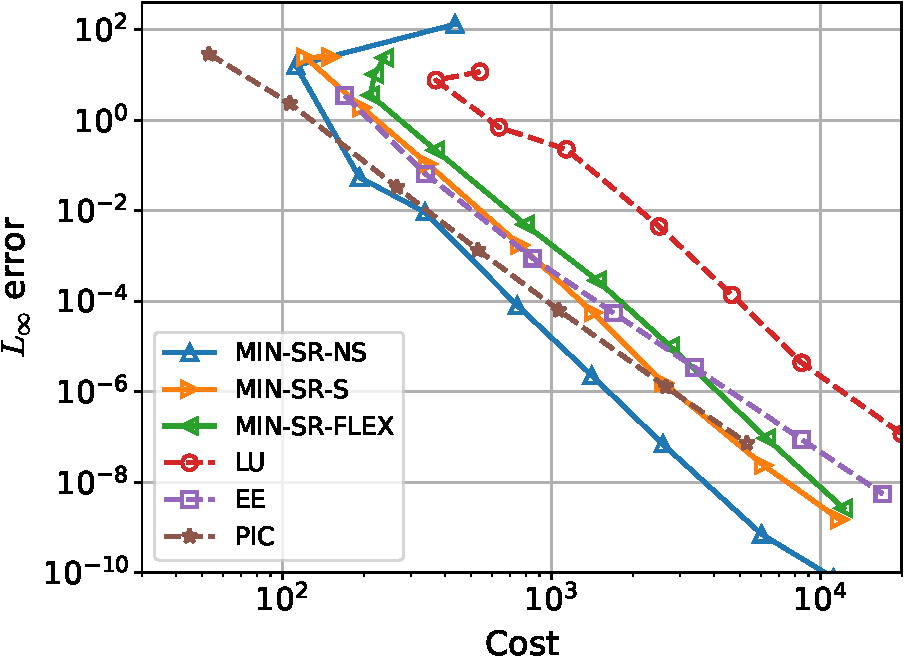
\includegraphics[width=0.5\textwidth]{fig1.pdf}}
\caption{Here is an example of a figure. Every figures must have a caption. Figure and caption should ideally already convey a lot of information to the reader, without having to consult the main body of the text. However, every figure must be discussed and interpreted in the text. If a figure is not referenced, delete it. The original figure appeared in a paper by Čaklović et al.~\cite{CaklovicEtAl2025}.}
\label{fig1}
\end{figure}

An example of a description of Figure~\ref{fig1} could roughly read:
Figure~\ref{fig1} shows the $L_{\infty}$ error against computational cost for the six studied methods.
For errors of around $10^{-1}$ or higher, the PIC method provides results with the smallest cost.
The MIN-SR-NS method has the smallest computational cost over the full range of errors from $10^{-1}$ down to $10^{-10}$.
This supports our claim that MIN-SR-NS is the most efficient solution algorithm, except for simulations where only very low precision is required.

%%
%%
\section{Structure of your thesis}
A typical structure would be
\begin{enumerate}
 \item Introduction
 \item Methodology
 \item Results
\end{enumerate}
This, however, is not set in stone and there is some flexibility.
For example, some prefere to have a section that results that is purely descriptive followed by another section that discusses and interprets results.
That is fine!
You do not necessarily require a conclusion section but can add one if you prefer.

\paragraph{Feedback} We will give you feedback on your writing before you submit.
This will be discussed in our supervision meetings but ideally you will submit an early sample of your writing (e.g. a description of your research question and methodology) and a more complete sample closer to your submission deadline.
If we have improvements on your structure, we will say so in our feedback.

%%
%%
\section{Your defence}
We will find a day and time for your defence as the submission deadline approaches.
It will typically take place in the E-10 institute.
Your defence will consist of a presentation by you, following by a question \& answers session.
The invitation for your talk will go out to the members of the Institute of Mathematics.
However, in most cases, the audience will be fairly small.

\paragraph{Your presentation}
The presentation at your defence \emph{must not exceed} 25 minutes.
If necessary, we will interrupt your talk.
Please use the template of the TUHH presentation for your talk~\cite{tuhh}.

%%
%%
\section{Supervision}
We will typically schedule a weekly meeting of up to one hour.
However, most of the meetings will not last that long and we certainly do not expect you to have one hour worth of new results every week.
If you do not have anything to discuss, you may always cancel the meeting, even on short notice. 
Meetings can be held either in person or via Zoom.
Do not hesitate to ask for a meeting to be moved to Zoom if this becomes necessary because of personal circumstances, e.g. illness or caring duties.

We will give you feedback on your write-up at least twice during your project.
The first round of feedback will be relatively early on, typically when you have decided on the mmethodological approach that you want to use.
At this stage, we will ask you to write a first draft of your methodology section and provide feedback on that.
Do not worry if this is still a very rough draft, the idea is to flag any important issues in your writing early.

A second round of feedback will be towards the end when your thesis is already mostly complete and the majority of your results is included.
%%
%%
\section{Reproducibility}
Almost every thesis written in our group will involve writing software.
This software is an inherent part of your project - however, in your thesis, you will have to focus on explaining the algorithms, in most cases you will not have space to talk about the implementation.
To ensure reproducibility of your results, you \emph{must} upload your code to TUHH's GitLab and give your examiners access to the repository, so that we can verify your results.
Sharing code used to produce research results is an important part of good scientific practice and required by research agencies like Deutsche Forschungsgemeinschaft (DFG).

%%
%%
\section{Why we are doing this to you}
You will most likely struggle to fit your results into the limited scope of a paper.
This is normal and arguably true for any scientific paper that was ever written!
It might help you to look at some papers that were written by doctoral researchers of our group~\cite{IbrahimEtAl2023,IbrahimEtAl2025,JohnEtAl2026}.

The reason we require this short format is largely a reaction to the easy availability of LLMs.
A detailed description even of some relatively arcane neural network architecture or numerical method can by now generated quickly using so-called AI.
We have no interest in assessing your capabilities in submitting text produced by ChatGPT -- we want to grade your skill in scientific thinking and writing.
By being forced to carefully decide which of your results are important and how you can link claims and evidence in extremely concise form, you will  be forced to think deeply about your topic!

\bibliographystyle{IEEEtran}
\bibliography{references}



\end{document}
